\documentclass{beamer}
\usepackage{graphicx}
\usepackage{pgfpages}

\usetheme{default}
\setbeamercolor{normal text}{bg=white!10}


\author{Prateek \\ Advisor: Puru}
\title{KVM Memory Optimizations}

\subtitle{\large{\emph{\alert{Improving Memory-management with KSM}}}}
\date{September 24, 2011}
%\advisor{Puru}
%\setbeameroption{show notes}
%\setbeameroption{show notes on second screen}
\begin{document}

\begin{frame}
 \maketitle
%\textbf{Increasing memory density with KSM, \emph{and more}}
\note{}
\end{frame}

\begin{frame}
 \frametitle{High-Level Goals}
\begin{itemize}

\item \alert{Increase number of VMs without degrading performance.}

\item Improve how guests (and hosts) utilize physical memory.
\item \alert{Why Memory :} Most constrained and non-renewable resource.
\item Allocated to guests at their boot time.
\item Memory overcommit is one of the key drivers of virtualized hosting
\item \emph{Everyone wants 8GB, even if they are using a few MB}   
\item Dynamic memory management in VMMs using page-sharing.
\item \textbf{KSM = Kernel Samepage Merging}

\note{ The main motivation is obviously to increase the number VMs that we can pack into a single physical machine. I guess that's everyone's goal here. 
For my project, i am looking at how memory utilization can be improved in virtual systems.  I think that memory is (still) the main bottleneck for most computer systems. 
And thats primarily because of the increasing costs of fetching a page from disk. Also, overcommitting memory is one the key benefits of virtualiztion. If we dont overcommit resources, why even virtualize? }
\end{itemize}
\end{frame}


\begin{frame}
  \frametitle{Page-Sharing}
Assume pages X and Y have same content. 
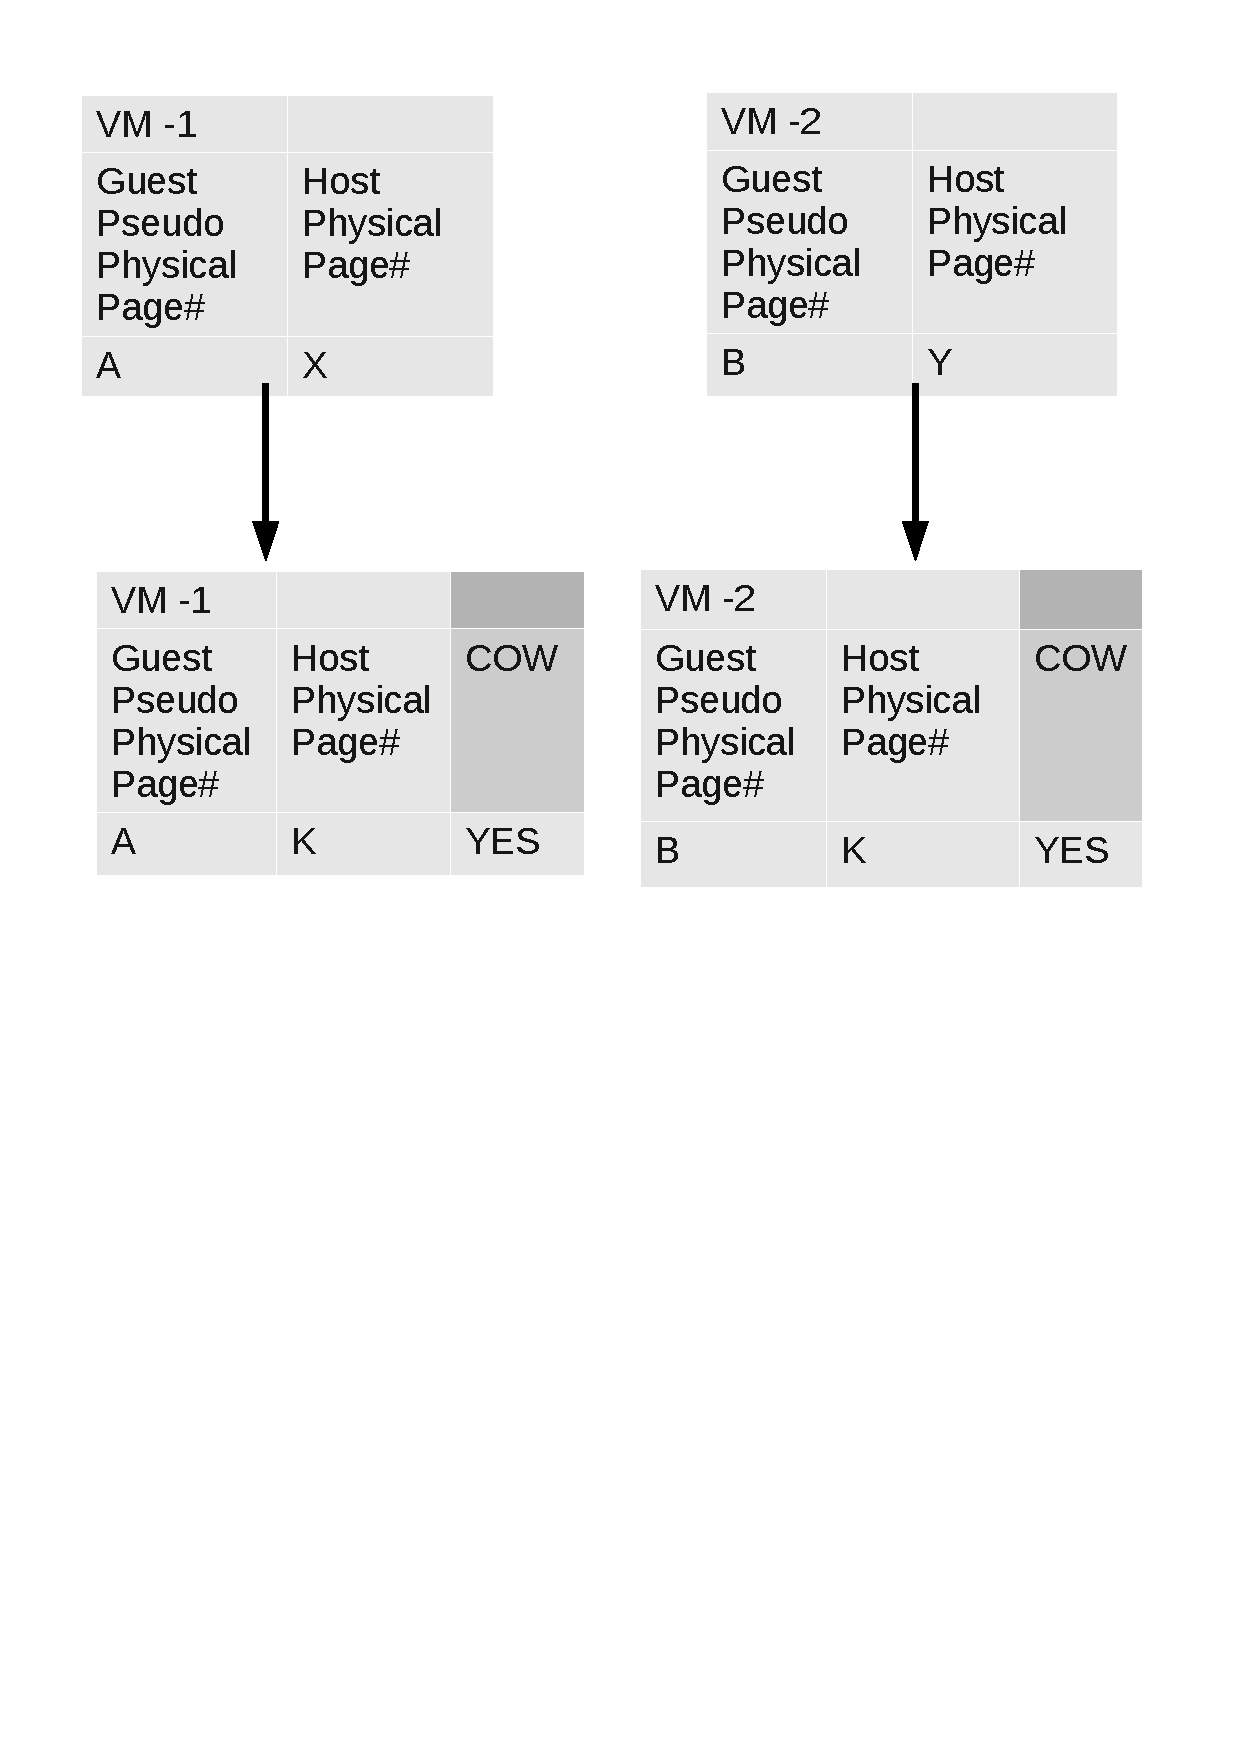
\includegraphics[scale=0.5]{PTE.pdf}

\note{So, how do we provide memory overcommitment without performance loss? One deterministically 'safe' way is to by using page sharing. I am looking primarily at KVM , and KVM does page-sharing by using the KSM, which is a functionality implemented in the linux kernel itself. The idea behind page sharing is simple: pages with same content can be replaced by a single page. All these shared pages are marked copy-on-write, so we are guaranteed safety.
DIAGRAM COMES HERE
}  
\end{frame}

\begin{frame}
\frametitle{KSM \& Page-Sharing}
\begin{itemize}
  \item \alert{KSM } implements \emph{Content Based Page Sharing} in linux.
  \item Multiple pages with the same content are merged into one.
  \item Detects similarity among ever-changing objects(pages)
  \item Brute-force search at regular intervals : scanning.
  \item Different implementations : VMWare ESX, Difference Engine, Satori, KSM.  
\end{itemize}

\alert{This talk: Describe 3 modifications to KSM }
\note{I am primarily working on KVM, so i'll be covering page-sharing from a KVM perspective. KVM uses the KSM to implement page sharing. 
KSM has been the target of my focus all this while, so i'll take a little time to describe it's operation. }

\end{frame}


% \begin{frame}
%   \frametitle{This talk}
%   \item Improve KSM
%   \item Use it to improve page-cache utilization
% \end{frame}


%%%%%%%%%%%%%%%%%%%%%%%%%

\begin{frame}
  \frametitle{KSM operation}\vspace{-13mm}
 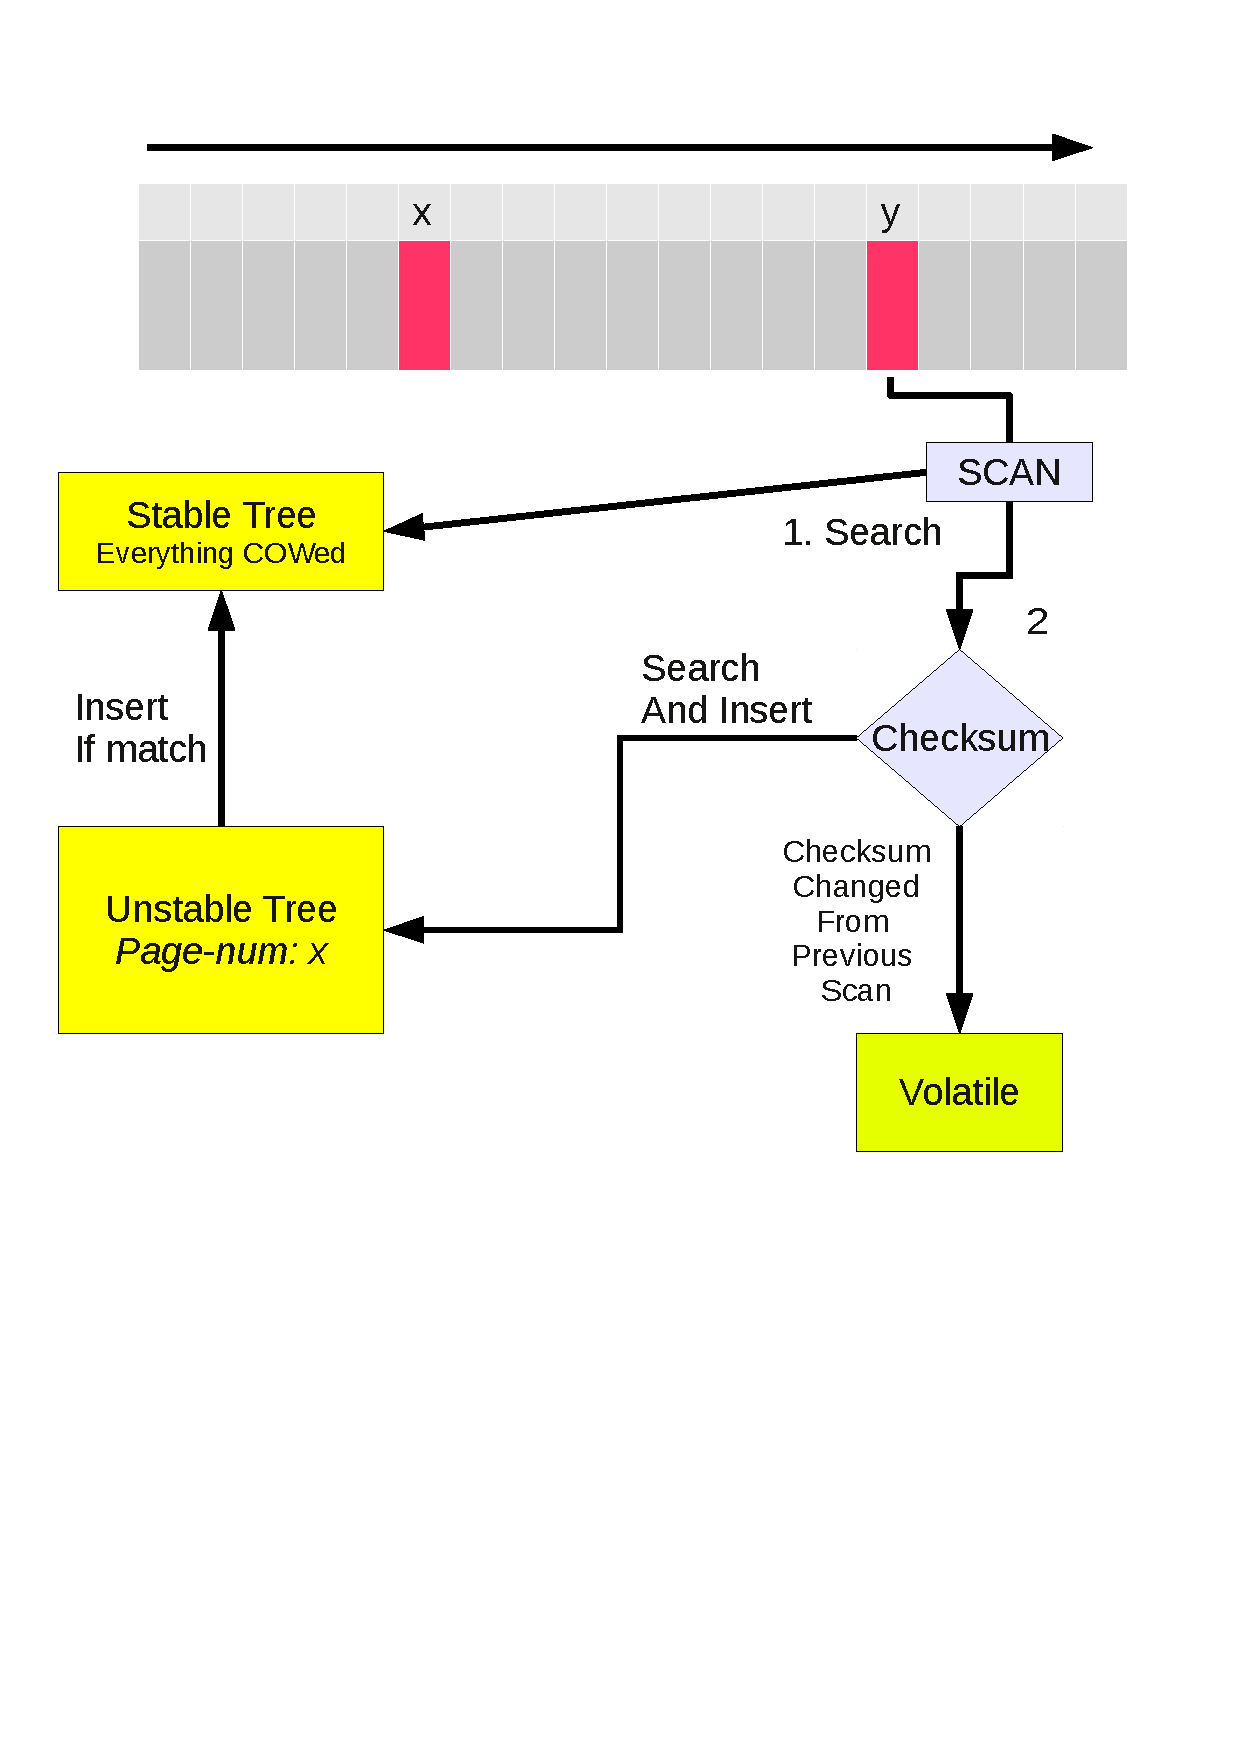
\includegraphics[scale=0.5]{KSM_operation.pdf}
\end{frame}

\begin{frame}
\frametitle{KSM}
\alert{The Good:}  
  \begin{itemize}
  \item Very general and non-disruptive solution - meant for page sharing in arbitrary memory areas.
  \item Any \texttt{malloc}'ed area is shareable (via \texttt{VM\_MERGEABLE})
  \item Very few heuristics used.
  \end{itemize}
\alert{The Bad: }
\begin{itemize}
  \item Significant overhead due to continuous scan+compare
  \item 10-20 \% CPU utilization in most cases.
\end{itemize}
\alert {The Ugly :}
\begin{itemize}
\item Design constrained by a patent minefield.
\end{itemize}

\end{frame}

\begin{frame}
  \frametitle{Lookahead}
  \begin{itemize}
  \item Shared pages in VMs are contiguous (seen using \texttt{ftrace})
  \item Lots of shared pages are file-backed. (guest \texttt{kpageflags})
  \item Modify KSM search to account for this spatial locality
  \item \alert{Peek at next page before doing the tree-search}
  \item Assuming consecutive shared pages occour with probability  p , Reduce search costs from log(u) to (1-p)log(u) + (p)1.
  \end{itemize}
\end{frame}


\begin{frame}
  \frametitle{Lookahead}
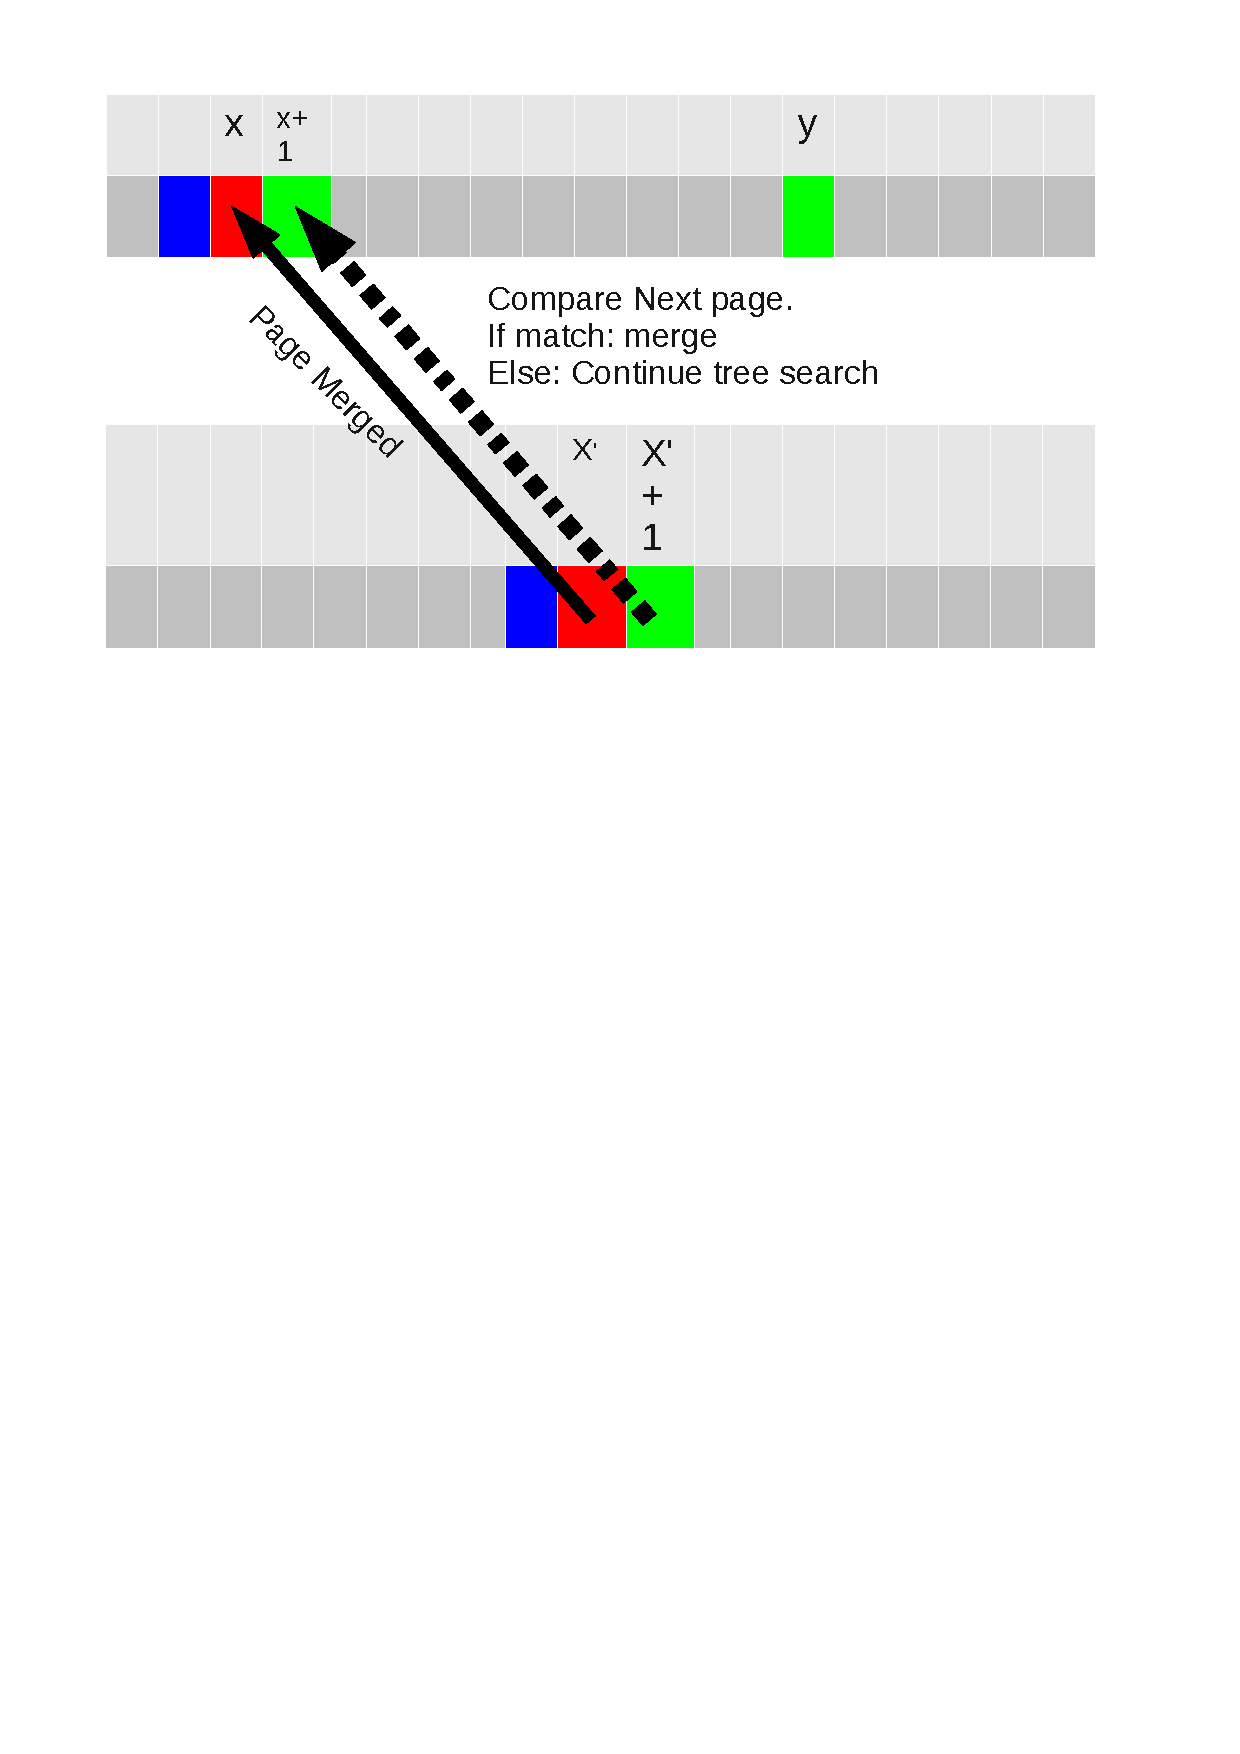
\includegraphics[scale=0.6]{Lookahead.pdf}
\end{frame}

\begin{frame}
  \frametitle{Lookahead}
  \begin{itemize}
  \item Lookahead optimization has no overhead in the worst case.
  \item Shared pages \textbf{increase} because KSM can scan lot more pages per CPU cycle.
  \item Ideal situations: sharing of large files.
  \item Desktop environments are best. (X11 fonts, programs, etc). 
  \item Sub-optimal situations: Lots of sharing, but fragmented. (Kernel compile)
  \end{itemize}
\end{frame}


\begin{frame}
  \frametitle{Lookahead results}
\begin{table}
\begin{center}
\begin{tabular}{|p{2cm}|p{2cm}|p{2cm}|p{1.2cm}|p{1.2cm}|}
\hline
 Workload (2VMs)  &  Avg. Shared Pages - Vanilla  &  Avg. Shared Pages - lookahead  &  CPU-look  &  CPU-Vanilla  \\
\hline
 Boot up          &  8,000                        &  11,000                         &        12  &           12  \\ \hline
 Kernel Compile   &  26,000                       &  30,000                         &        22  &           19  \\ \hline
 Desktop VM use   &  31,000                       &  62,000                         &      16.8  &         14.6  \\ 
\hline
\end{tabular}
\caption{Lookahead performance}
\end{center}
\end{table}

Average shared pages (over time) during the course of the workload.  \\
CPU usage is also the average over time. 

\end{frame}



\begin{frame}
  \frametitle{QEMU IO}
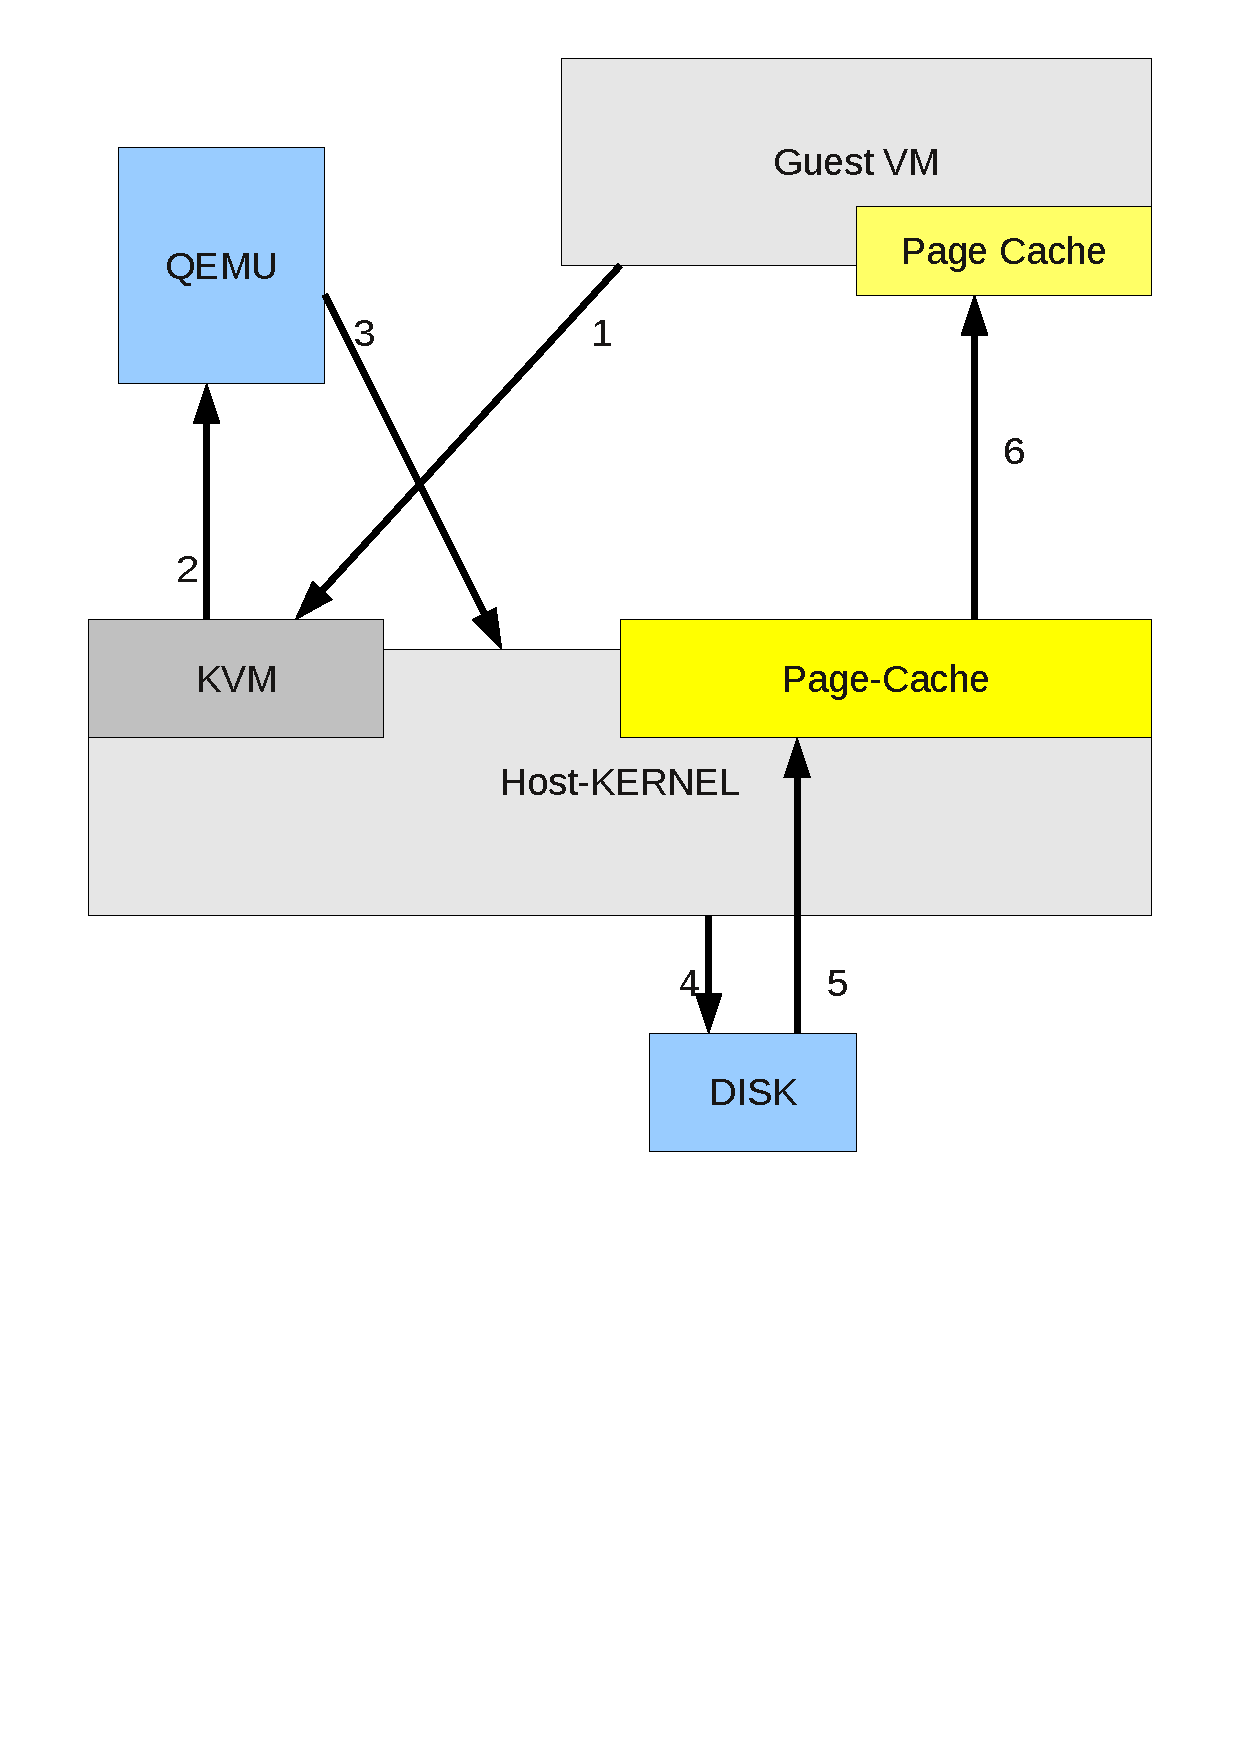
\includegraphics[scale=0.40]{qemu.pdf}

\end{frame}

\begin{frame}
  \frametitle{Exclusive Caching}
  \begin{itemize}
  \item All guest disk IO goes through host page-cache.
  \item Double-caching : Same block is present in both host and guest caches.
  \item Ideally a block should be present in either of the caches.
  \item Exclusive caches are known to provide better cache utilization. [See: Geiger, gill, mycacheyours].
  \item Mounting virtual disks as \texttt{O\_DIRECT} adds too much penalty.
  \item No solution to this for KVM-like systems exists \ldots

  \end{itemize}
\end{frame}

\begin{frame}
\frametitle{Host memory cache pollution with \texttt{yes} workload}
  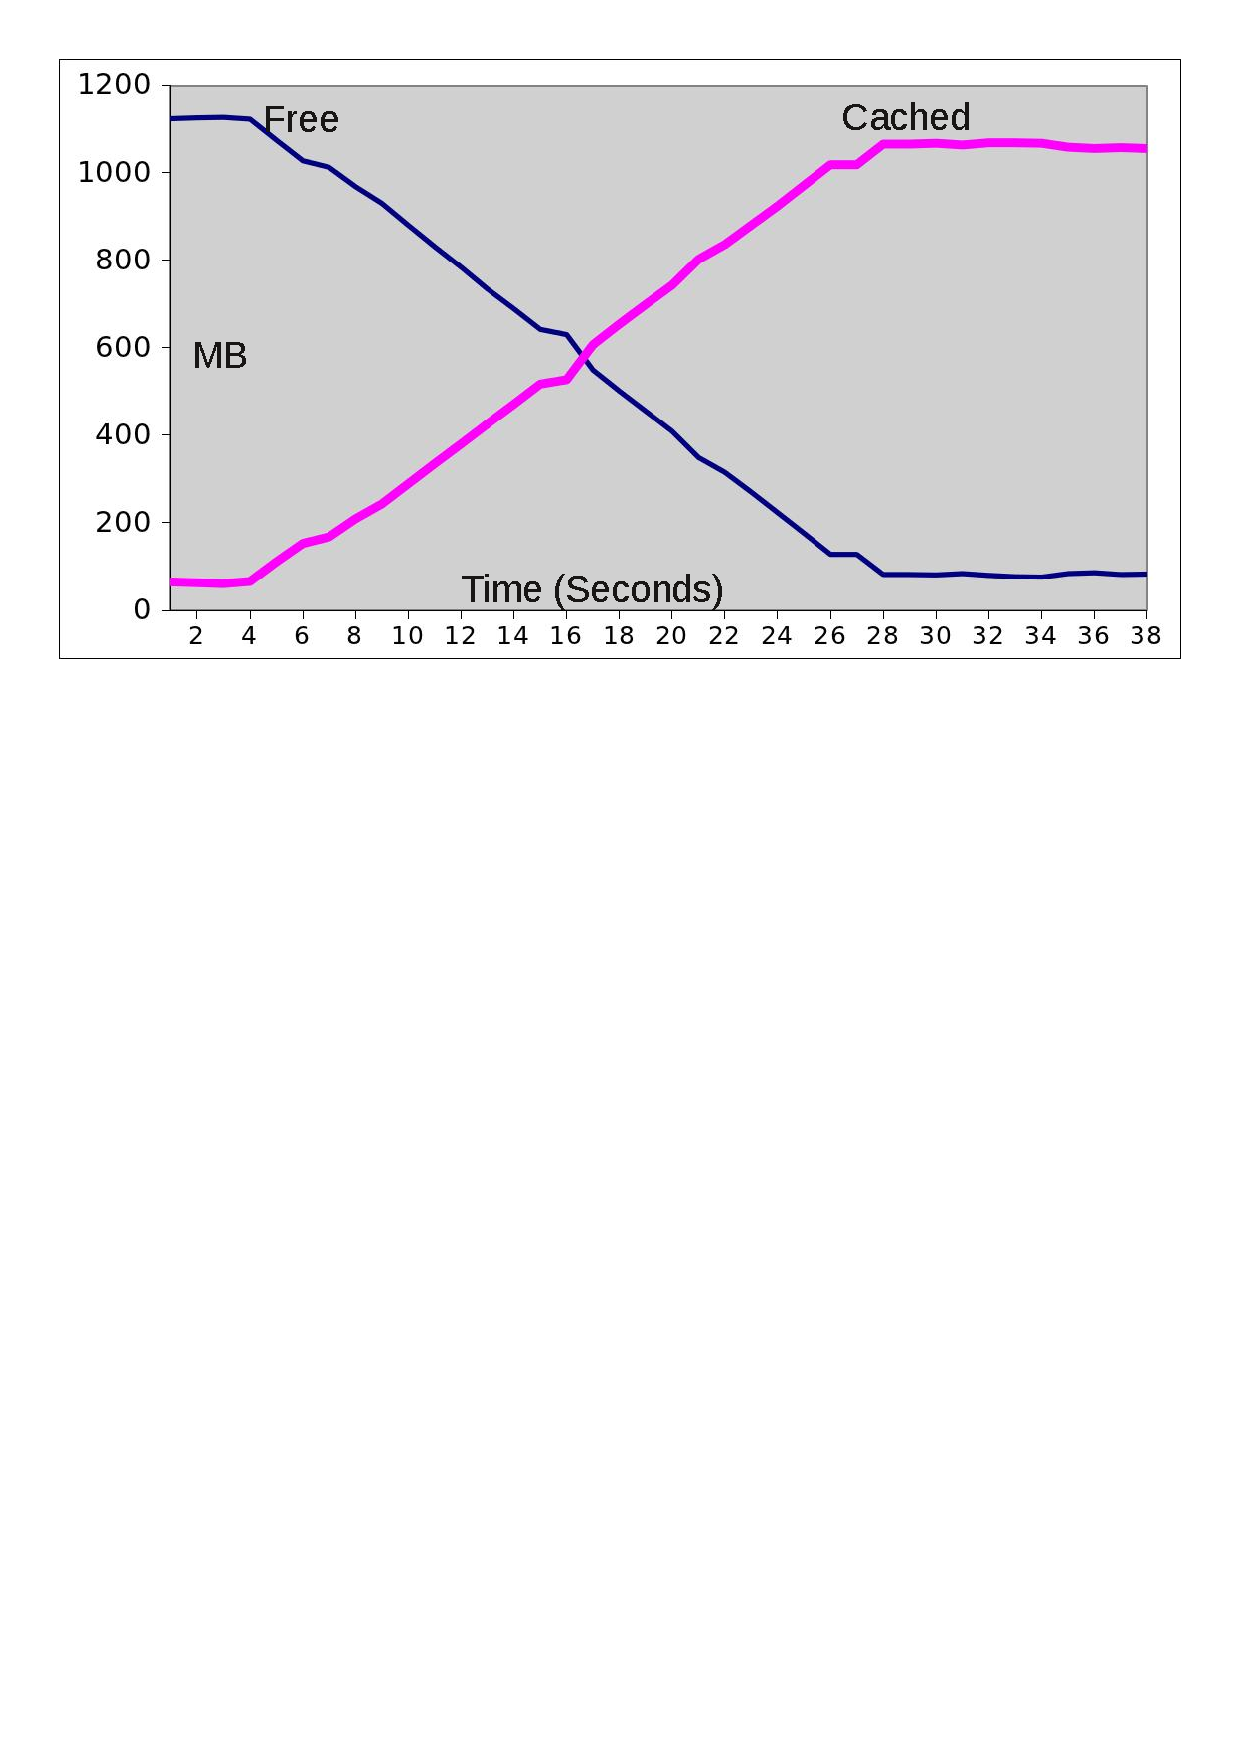
\includegraphics[scale=0.55]{yes2.pdf}
\end{frame}

\begin{frame}
  \frametitle{Double caching problem}
\begin{table}
\begin{center}
\begin{tabular}{|p{2cm}|p{1.6cm}|p{1.6cm}|p{2.0cm}|p{1cm}|p{1cm}|}
\hline
 \small{Workload  (2VMs)}      &  Avg. Shared Pages  &  Total Pages dropped  &  Avg Cache saved  &  CPU-ksm  &  CPU-exc  \\
\hline
\small{Kernel Compile(2 GB)}  &  75,000             &                       &  \small{512M - 260M}      &       14  &       16  \\
\small{Desktop VMs}        &  62,000             &  162,000              &  \small{400M- 219M}       &     18.8  &     14.6  \\
\hline
\end{tabular}
\caption{Exclusive Cache benefits. Significant reduction in host page cache size. Increased CPU usage due to cache scrubbing.}
\end{center}
\end{table}
\end{frame}

\begin{frame}
  \frametitle{Exclusive Caching}
  \begin{itemize}

  \item {Wasting memory by caching 2 copies clearly wasteful}
  \item {No existing solution for virtual setups}
  \item \alert{Use KSM!}
  \item Drop a page from host page-cache if it's already present in guest.
  \item Luckily for us, KSM builds a nice search tree of all guest pages!
  \item Scan at the end of every KSM pass, comparing host page-cache pages with unstable,stable tree.
 \item If match found, drop page from host cache
 \end{itemize}
\end{frame}

\begin{frame}
  \frametitle{Evaluation of Exclusive Cache}

\begin{table}
\begin{center}
\begin{tabular}{|l|l|l|}

\hline
 Test          &  Plain       &  With Excl Cache  \\
\hline
 Write(char)   &  24,000 K/s  &  32,000 K/s       \\
 Read(char)    &  27,000 K/s  &  27,500 K/s       \\
\hline
 Read(block)   &  53,750 K/s  &  47,700 K/s       \\
 Write(block)  &  22,500 K/s  &  23,800 K/s       \\
\hline
\end{tabular}
\caption{Exclusive cache impact on Bonnie++ benchmark. Executed on 2 VMs. }
\end{center}
\end{table}

\begin{itemize}
\item The caches are not scrubbed often enough in this short-lived benchmark
\item Nevertheless significant performance gains
\end{itemize}

\note{IOZONE?}
\end{frame}

\begin{frame}
  \frametitle{Cache scrubbing in action}
Free and Cached memory (in MB) for a sample Bonnie workload. \\
Obsserve the page-dropping at regular intervals. \\
  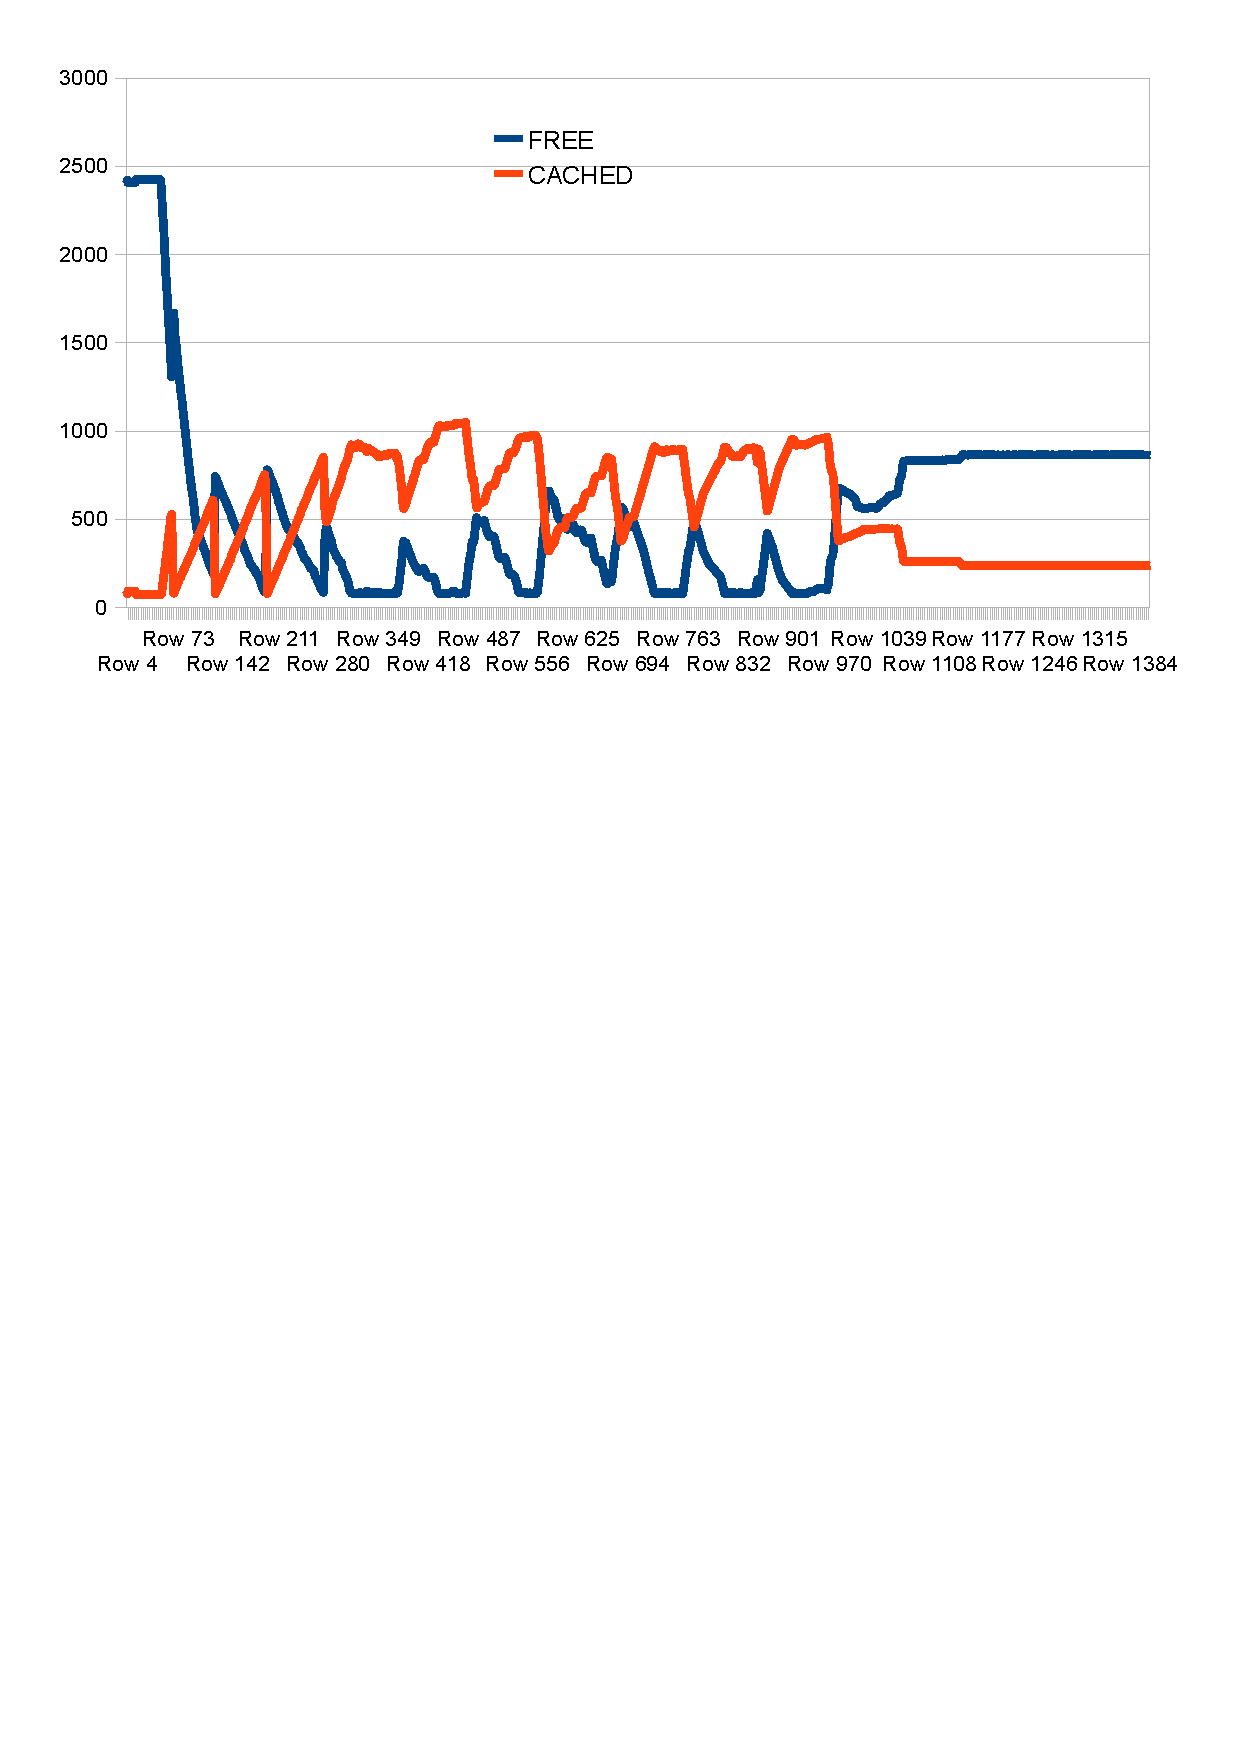
\includegraphics[scale=0.5]{battle.pdf}
\end{frame}

\begin{frame}
  \frametitle {Kernel-hacking timeline}
  \begin{table}
    \centering
    \begin{tabular}{lc}
      KSM page-flags & 1 Month (!) \\
      Ftrace instrumentation & 2 days\\
      Lookahead implementation  & 3 weeks  \\
      Exclusive Cache implementation & 2 hours  \\ 
    \end{tabular}
    \caption{Time spent}
  \end{table}

  \begin{itemize}
  \item Currently on kernel version \textbf{195} (number of times compiled)
  \item Compile $\rightarrow$ Reboot $\rightarrow$ Debug cycle is exhausting.
  \item Tricks : QEMU gdb mode , kexec , ksplice. 
  \item The kernel infrastructure is \emph{amazing} :  \texttt{Lockdep} (detect deadlocks!) , \texttt{kmemcheck} , \texttt{debug\_info} \ldots
  \end{itemize}

\end{frame}

\begin{frame}
  \frametitle{TODO}
  \begin{itemize}
  \item More experiments, with different workloads.
  \item Need low-intensity, high-sharing benchmarks. 
  \item Zipf workload comparison with truly exclusive vs. KSM-exclusive vs. Drop-all.
  \item Implement WSS estimator using KSM. (detect evictions).
  \item More KSM improvements to be tested .
  \end{itemize}
\end{frame}




\begin{frame}
  \frametitle{Page Sharing by Flags}
\begin{itemize}
  \item Hypothesis: Sharing page-cache pages is bad.
  \item Page-cache pages are overwritten frequently anyway.
  \item Page-cache size is 50\% of available memory , so significant KSM savings.
  \item This hypothesis turns out to be \emph{wrong} 
\end{itemize}
\end{frame}

\begin{frame}
  \frametitle{Implementation}
  \begin{itemize}
  \item Guest writes its page-flags into a memory hole. 
  \item Host (KSM) needs to access statically defined address in the guest. \alert{HOW?}
  \item Kernel doesnt seem to have a mechanism to provide memory by physical addresses
  \item \alert{Currently :} Create memory-hole at boot-time and write to it (using \texttt{ioremap} )
  \end{itemize}
\end{frame}



\end{document}
